\section{Adaptive Bitrate Streaming}\label{sec:adaptive_bitrate_streaming}
Multimedia streaming is a big part of the internet and many optimizations have
been developed to improve the quality of service for the end-users.
This includes considering (in real-time) parts of the clients connection state, 
such as available bandwith, and adapting the rate at which a server sends data.
Such a process is called `Adaptive Bitrate Streaming' and is employed in many 
of todays streaming setups.
An example setup can be seen in~\autoref{fig:adaptive-bitrate-streaming} where
within the content delivery network multiple streams with different resolutions
exist and the edge server that manages the connection to the client can switch
between those streams based on the clients connection state.
Youtube and Netflix are examples where, although more complex, similar setups
are used to provide a better user experience. 
% TODO: cite    https://netflixtechblog.com/optimizing-the-netflix-streaming-experience-with-data-science-725f04c3e834
% TODO:         https://www.cloudflare.com/de-de/learning/video/what-is-adaptive-bitrate-streaming/
% TODO:         https://docs.imagekit.io/features/video-transformation/adaptive-bitrate-streaming

\begin{figure}[htbp]
    \centering
    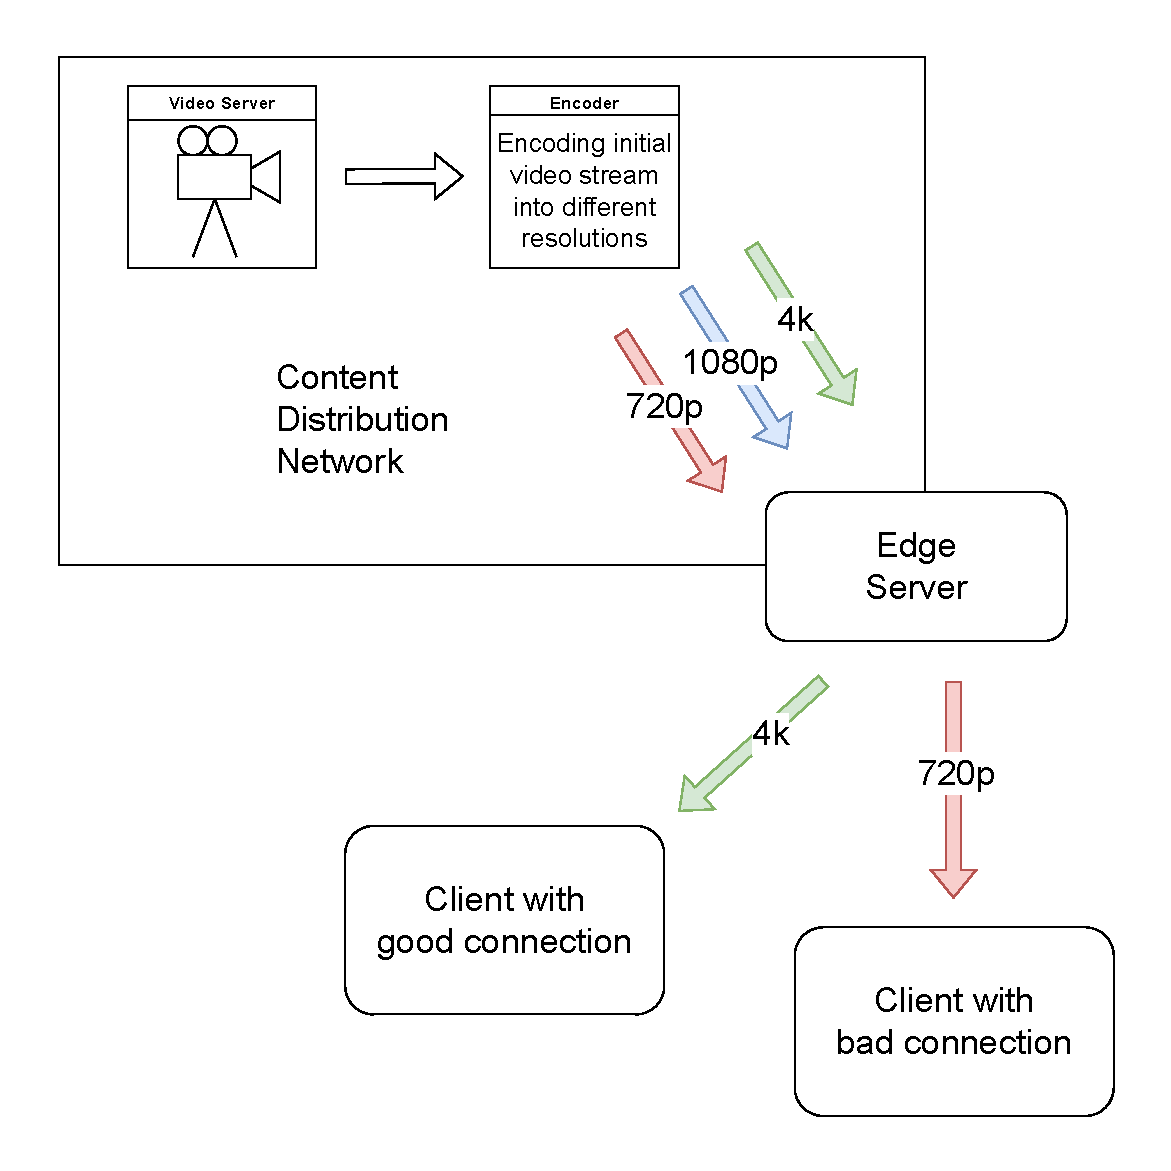
\includegraphics[width=7cm]{figures/02_background/adaptive-bitrate-streaming.drawio.pdf}
    \caption{A streaming server might send multiple streams with different
    resolutions to allow adapting to a users bitrate.}\label{fig:adaptive-bitrate-streaming}
\end{figure}

The way the example implementation of fast-realys in this thesis is set up,
is that the video server will encode into each packet its priority.
For example I-frames have a high priority while P-frames have a lower
priority.
The relay then can decide not to forward certain packets to a client if
the client is experiencing congestion.

TODO more specifics on how client state is found out.